% TEMPLATE for Usenix papers, specifically to meet requirements of
%  USENIX '05
% originally a template for producing IEEE-format articles using LaTeX.
%   written by Matthew Ward, CS Department, Worcester Polytechnic Institute.
% adapted by David Beazley for his excellent SWIG paper in Proceedings,
%   Tcl 96
% turned into a smartass generic template by De Clarke, with thanks to
%   both the above pioneers
% use at your own risk.  Complaints to /dev/null.
% make it two column with no page numbering, default is 10 point

% Munged by Fred Douglis <douglis@research.att.com> 10/97 to separate
% the .sty file from the LaTeX source template, so that people can
% more easily include the .sty file into an existing document.  Also
% changed to more closely follow the style guidelines as represented
% by the Word sample file. 

% Note that since 2010, USENIX does not require endnotes. If you want
% foot of page notes, don't include the endnotes package in the 
% usepackage command, below.

\documentclass[letterpaper,twocolumn,10pt]{article}
\usepackage{hyperref}
\usepackage{amsmath}
\usepackage{usenix,epsfig,endnotes}
\begin{document}

%don't want date printed
\date{}

%make title bold and 14 pt font (Latex default is non-bold, 16 pt)
\title{\Large \bf Path Planning with Imitation Learning}

\author{
{\rm Yiren Lu}\\
GRASP Lab, University of Pennsylvania\\
April 2016
}

\maketitle

% Use the following at camera-ready time to suppress page numbers.
% Comment it out when you first submit the paper for review.
\thispagestyle{empty}


\section{Introduction}

In ESE 650 5th project, we did path planning on University of Pennsylvania's high resolution (12480 $\times$ 5344) aerial photo with image processing, Dijstra's algorithm and imitation learning ~\cite{ratliff2009learning}. First, I extracted image feature maps using image processing techniques. And then, I used Dijstra's algorithm and imitation learning to iteratively learn the cost map from feature maps.
\begin{center}
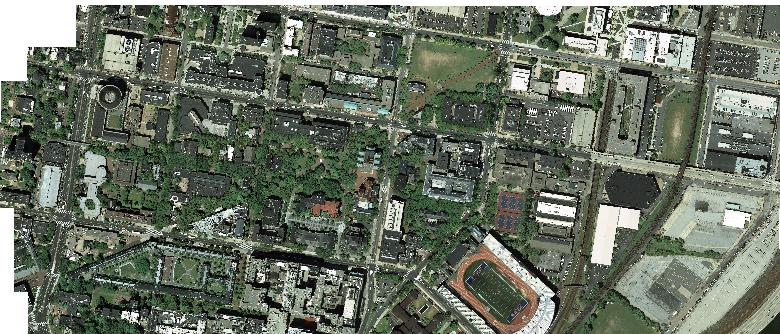
\includegraphics[scale=0.28]{imgs/aerial_color_d16.jpg}\\
\end{center}

\section{Dataset and Image Processing}

Since the aerial image is so big, I downsample the image by 8 and perform training and testing on that. Initially for this project, I used less-detailed feature set including RGB/HSV values, edges, and some GMM probability maps. However, the results are not as good as expected. Clearly, since the learning part largely depends on the features, they are critical to this project. Later I did more feature engineering. I thresheld with pixels of different color spaces, including HSV, L*A*B, YCBCR to separate green areas, roads, shadows and rooftops. More detailed feature maps were included in the $slides$ attached. Edges are good features for path planning, I used Canny, Prewitt and Sobel features. I also use kmeans algorithms to segment the map, and extraced nice side walk mask. On the other hand, I also extracted green areas, roads and buildings probability maps using Gaussian Mixture Model. \\

\section{Feature Maps}
By combining different feature maps together, I could basically reconstruct the area mask of driving and walking by hand designed features as shown in the images.\\


\begin{figure}[h]
    \centering
    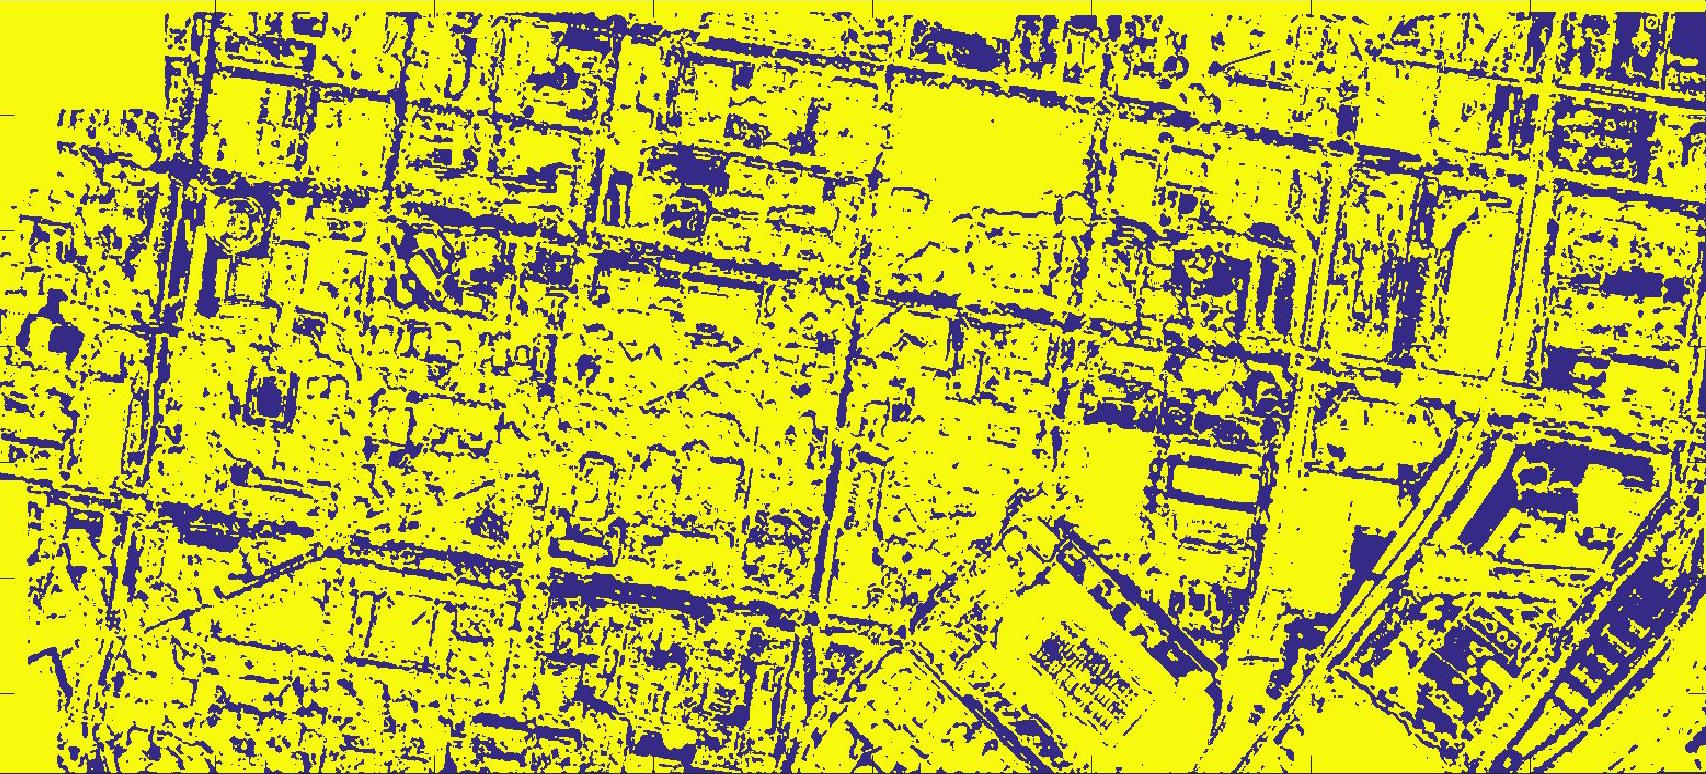
\includegraphics[width=0.5\textwidth]{results/all_driving.jpg}
    \caption{Drive area map}
\end{figure}

\begin{figure}[h]
    \centering
    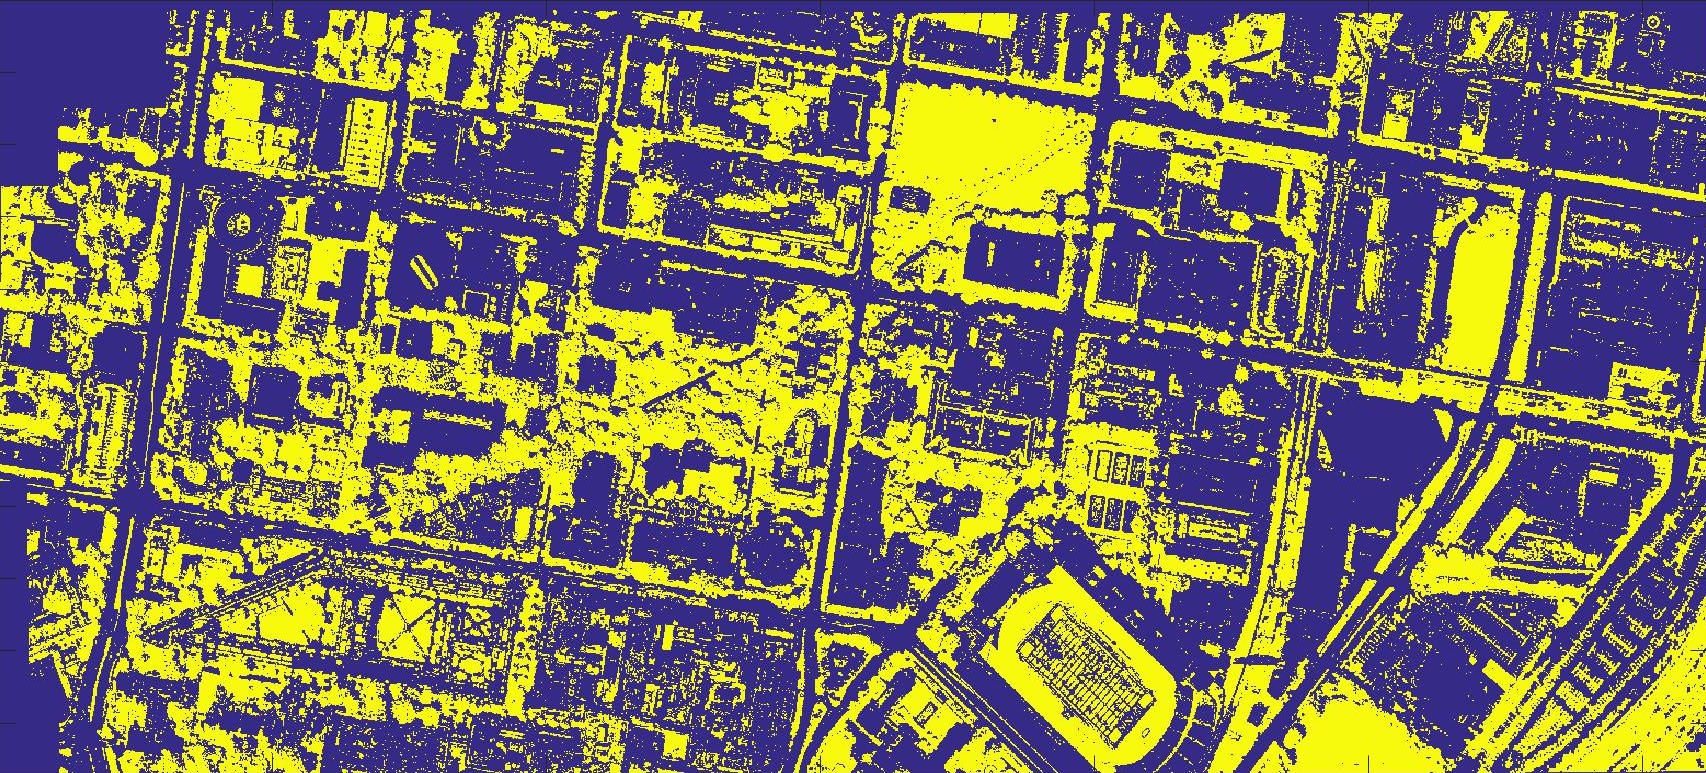
\includegraphics[width=0.5\textwidth]{results/all_greens.jpg}
    \caption{Walk area map}
\end{figure}



\section{Imitation Learning}
After extracted multiple feature maps, we then combine them by exponential of weighted sum. The basic path planning procedure is to compute the cost to go function using cost map by a dynamic programming approach, Dijstra's algorithm. And then use cost to go function to greedy plan the path. The cost function is defined by\\
\begin{align*}
C(x,y) = e^{\sum_{k=1}^K a_k F_k(x,y)} 
\end{align*}
Where, $a_k$ is the weight for the $k$th feature map $F_k$. Since in the practical learning process, the weights $a$ are not restricted to positive, but the Dijstra's algorithm can only take positive cost values, we exponentiated the cost map to make all the cost positive.\\
After that, I did gradient descent based imitation learning iteratively compute the optimal cost map.\\
\begin{align*}
\mbox{Minimize } J = \sum_{(x,y)^*} C(x,y)^* - \sum_{(x,y)} C(x,y)\\
\end{align*}
Where, $\sum_{(x,y)^*} C(x,y)^*$ is the total cost of the training path, $\sum_{(x,y)} C(x,y)$ is the tatal cost of the predicted path.\\
In order to learn the weights $a$, we used gradient descent method. \\
\begin{align*}
\frac{\partial J}{\partial a_k} =& \sum_{(x,y)^*} e^{\sum_{k=1}^K a_k F_k(x,y)^*} - \sum_{(x,y)}F_k(x,y)e^{\sum_{k=1}^K a_k F_k(x,y)}\\
\frac{\partial J}{\partial a_k} =& \sum_{(x,y)^*} C(x,y)^* - \sum_{(x,y)}F_k(x,y)C(x,y)\\
a_k = & a_k - \mu \frac{\partial J}{\partial a_k}\\
\end{align*}
For the training set, I labeled 30 samples for driving and 30 for walking. When I used less-detailed feature maps, the cost maps learning was as follows\\
\begin{center}
    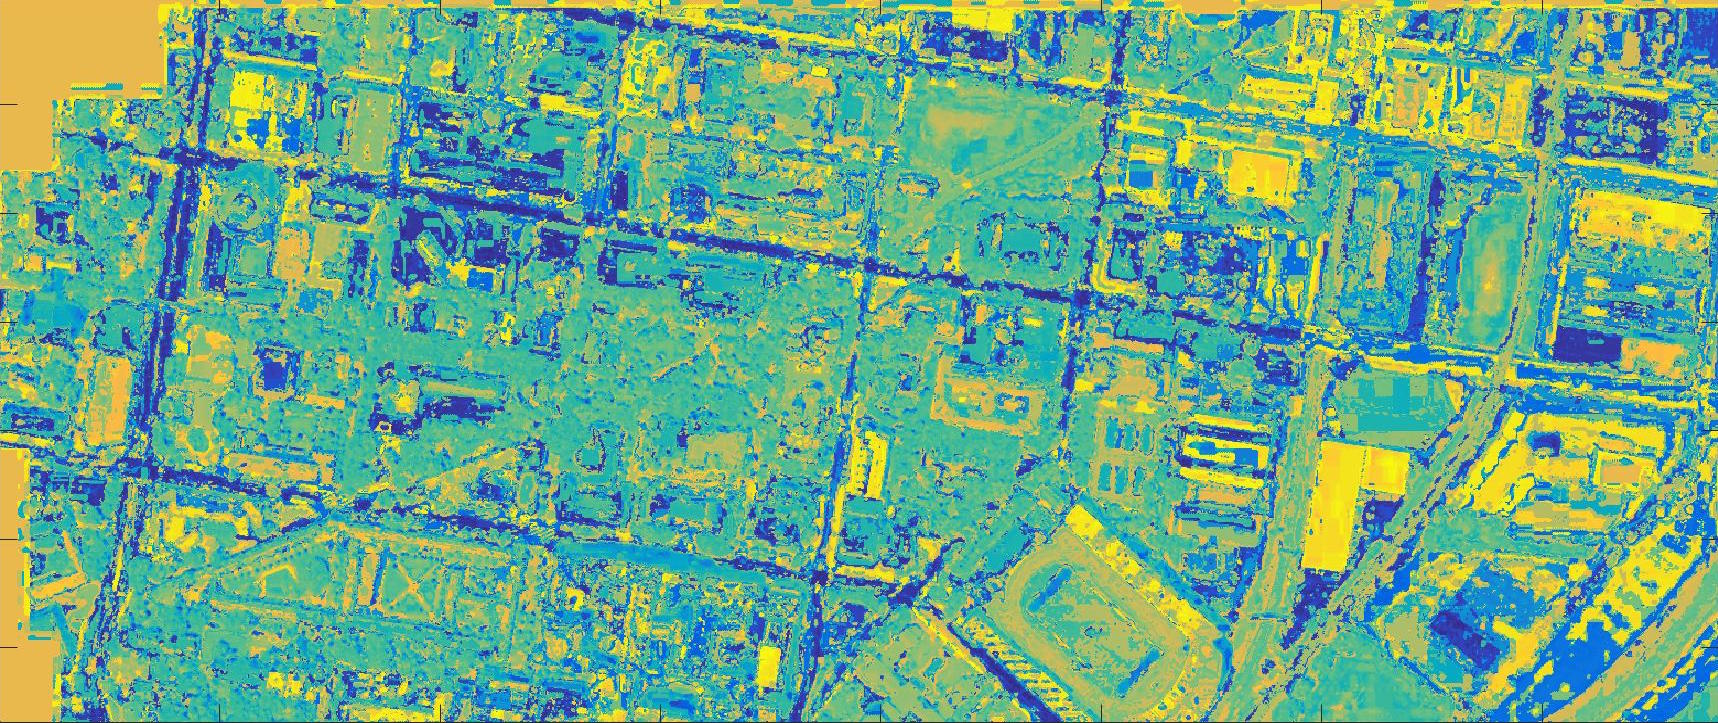
\includegraphics[width=0.5\textwidth]{results/featmap_apr3.jpg}
\end{center}
It basically worked, however, without detailed features about buildings, shadows, etc, the planner gives paths went across buildings from time to time. Further, I found that without stop criterion or early stop, the gradient descent tends to over fit the training data by zering out all the features with high cost under the predicted paths as well as lowering all the weights in order to obtain a lower cost.\\Since my hand-designed feature maps are similiar to the expected cost maps, the predicted paths quickly converged to the training paths.\\
For training, here are some tips\\
\begin{itemize}
\item I normalized the feature maps into between 0 and 1, since the initialization of features could largely influence the results of non-convex optimization.
\item The learning rate could vary for different setting of weights and cost maps.
\item Normalizing the weights in each iteration to some extent prevent overfitting.
\end{itemize}

\section{Results and Discussion}

\begin{itemize}
\item There is a bug in the given code getMapCellsFromRay.cpp, the output paths are always ordered by x from lower to higher, which is bad for applications requiring sequential order. I reimplemented this function and included it in the code submission $mex$ folder. 
\end{itemize}


\begin{figure}[h]
    \centering
    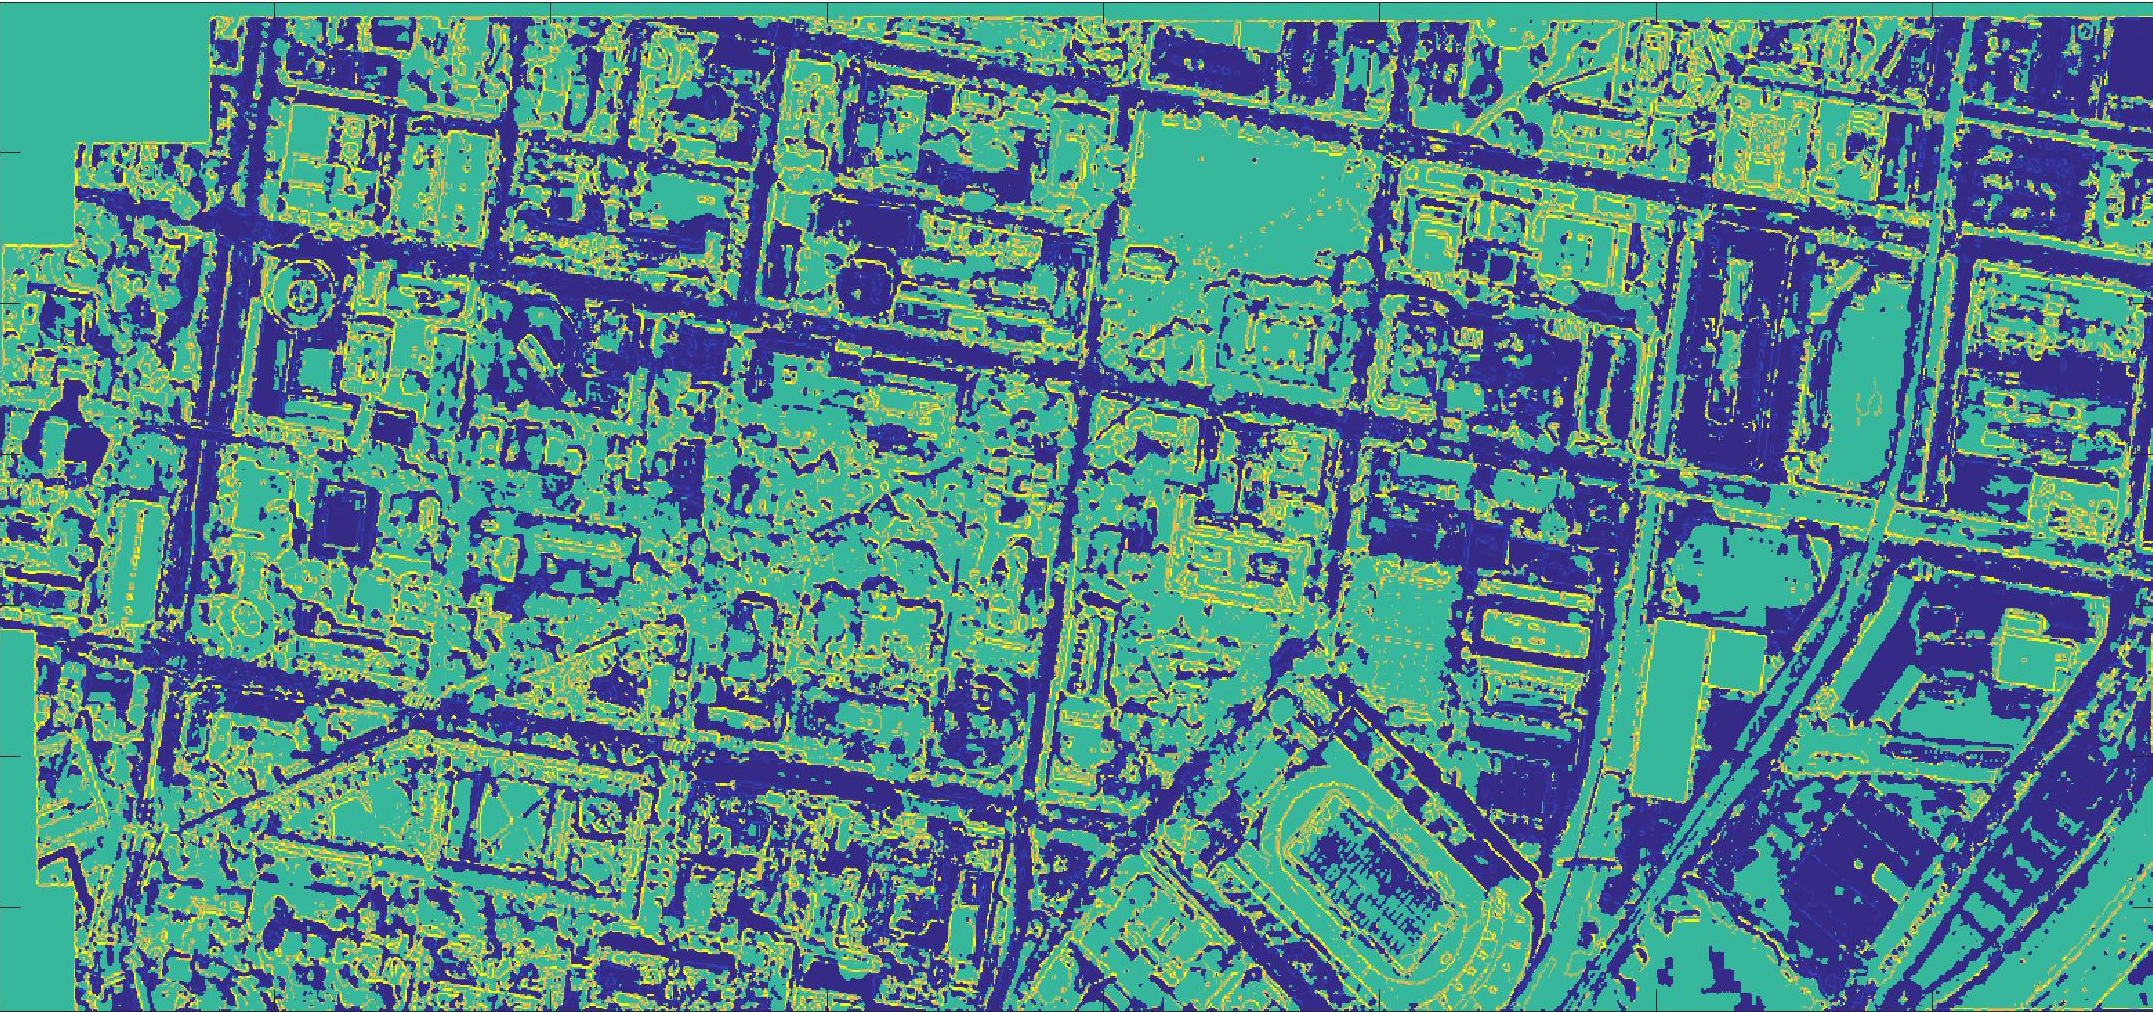
\includegraphics[width=0.5\textwidth]{results/cost_drive.jpg}
    \caption{Final cost map for driving}
\end{figure}

\begin{figure}[h]
    \centering
    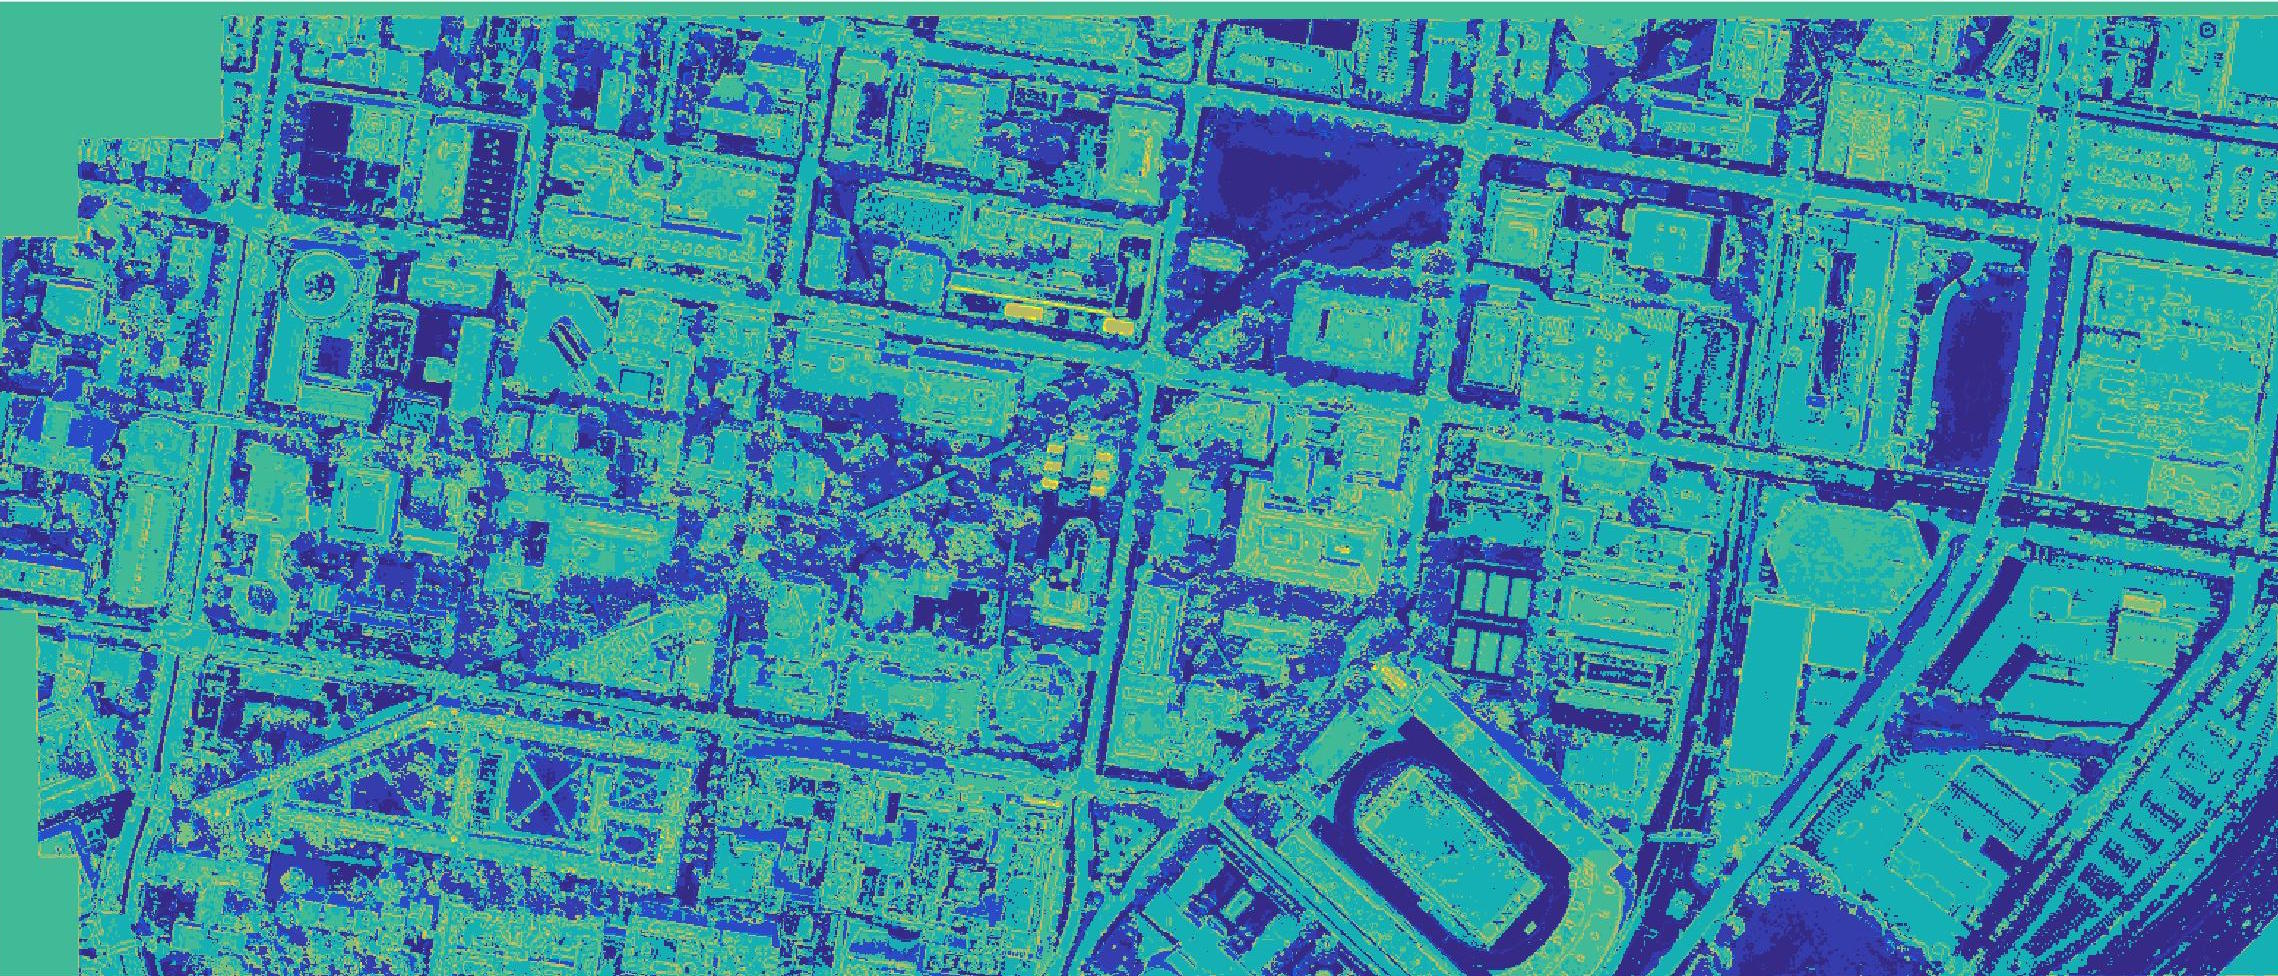
\includegraphics[width=0.5\textwidth]{results/cost_walk.jpg}
    \caption{Final cost map for walking}
\end{figure}


\section*{Acknowledgement}
Thanks Dr. Lee for designing and preparing this project and thanks TAs for timely responses to our questions.

{\footnotesize \bibliographystyle{acm}
\bibliography{sample}}



\begin{figure}[h]
    \centering
    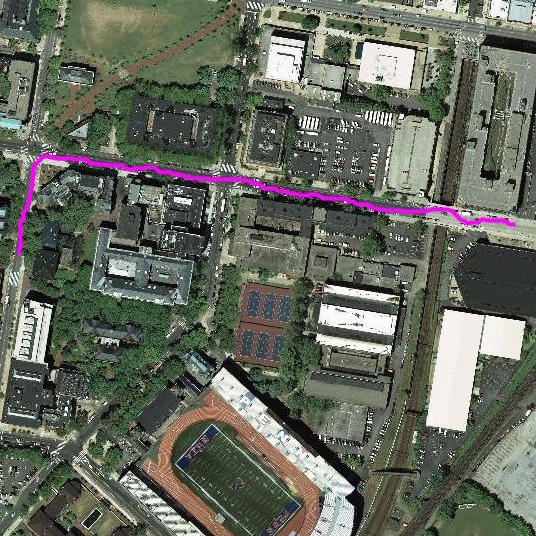
\includegraphics[width=0.3\textwidth]{results/test_drive1.jpg}
    \caption{Drive testcase 1}
\end{figure}

\begin{figure}[h]
    \centering
    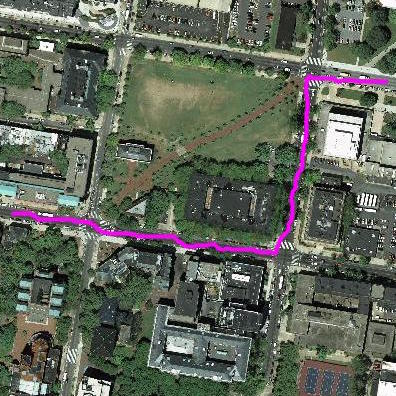
\includegraphics[width=0.3\textwidth]{results/test_drive2.jpg}
    \caption{Drive testcase 2}
\end{figure}

\begin{figure}[h]
    \centering
    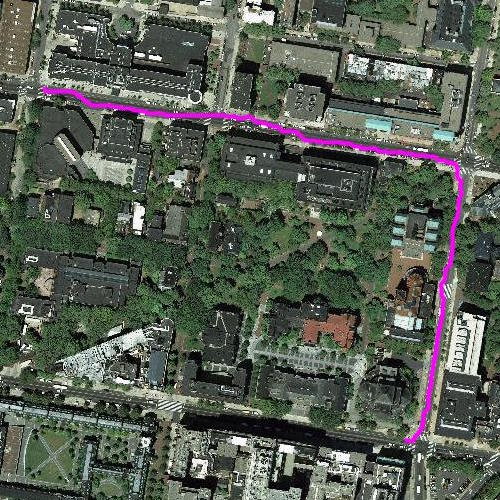
\includegraphics[width=0.3\textwidth]{results/test_drive3.jpg}
    \caption{Drive testcase 3}
\end{figure}

\begin{figure}[h]
    \centering
    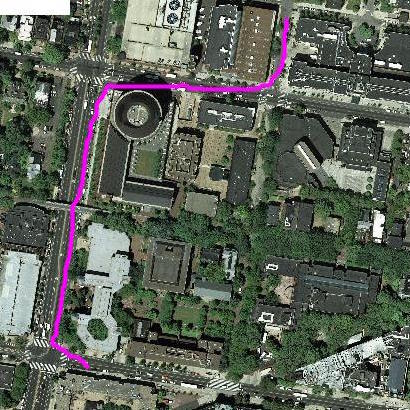
\includegraphics[width=0.3\textwidth]{results/test_drive4.jpg}
    \caption{Drive testcase 4}
\end{figure}

\begin{figure}[h]
    \centering
    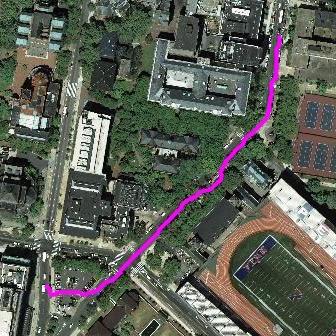
\includegraphics[width=0.3\textwidth]{results/test_drive5.jpg}
    \caption{Drive testcase 5}
\end{figure}

\begin{figure}[h]
    \centering
    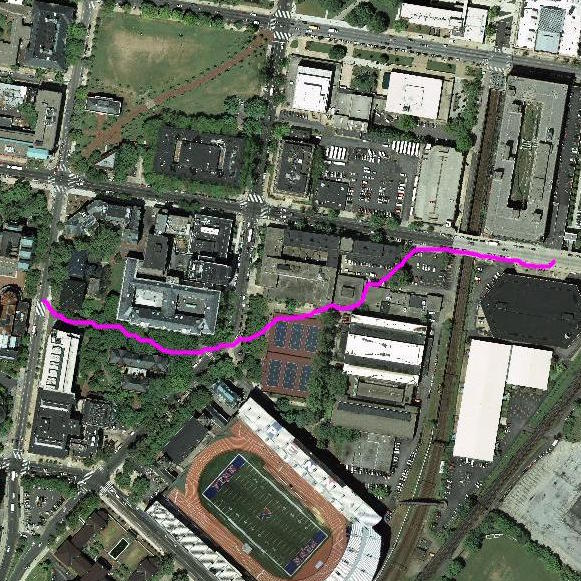
\includegraphics[width=0.3\textwidth]{results/test_walk1.jpg}
    \caption{Walk testcase 1}
\end{figure}

\begin{figure}[h]
    \centering
    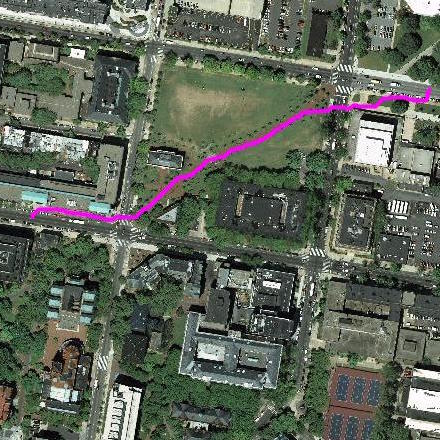
\includegraphics[width=0.3\textwidth]{results/test_walk2.jpg}
    \caption{Walk testcase 2}
\end{figure}

\begin{figure}[h]
    \centering
    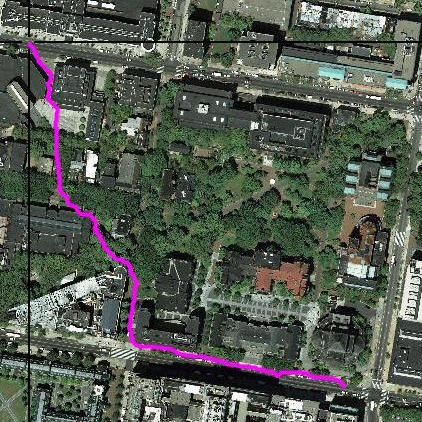
\includegraphics[width=0.3\textwidth]{results/test_walk3.jpg}
    \caption{Walk testcase 3}
\end{figure}

\begin{figure}[h]
    \centering
    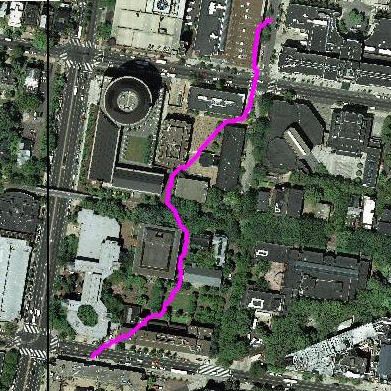
\includegraphics[width=0.3\textwidth]{results/test_walk4.jpg}
    \caption{Walk testcase 4}
\end{figure}

\begin{figure}[h]
    \centering
    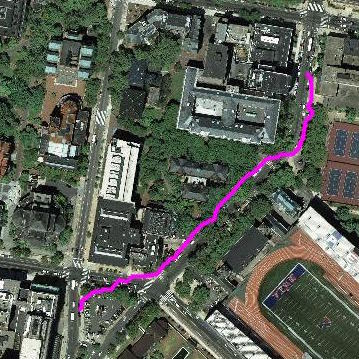
\includegraphics[width=0.3\textwidth]{results/test_walk5.jpg}
    \caption{Walk testcase 5}
\end{figure}


% \theendnotes

\end{document}







